\chapter{Software Design}
\label{chapter:04}
This chapter deals with the design of the software architecture on a high level and will describe the components of the ecosystem in which the package will fit in. Components may sometimes be referred to as classes and vice versa, \textit{component} being the general term and \textit{class} generally meaning the programming language feature equivalent of a component.

\section{System Design}
The core idea of the \textit{Mobility Feature Package} is to provide a very simple programming interface such that computing features can be done with very few lines of code. This requires closing of the internal working of the package off, such that the programmer has very limited ways in which he/she can interface with it. The design of the package API went through two main iterations which consisted of many smaller iterations. Mainly, the difference between the final iteration and the earlier iterations is the amount of code required for managing historical data that the programmer has to write. Early iterations put the responsibility on the application programmer to manage historical data. After developing the field study app discussed in chapter \ref{chapter:06} it was decided to move most of this logic inside the package; it became glaringly apparent that the package was too cumbersome to use. The final iteration is the one discussed in this thesis including the choices and lessons learned on the way of designing and developing it. The flowchart in Figure \ref{fig:flowchart-features} displays the task which the software system must be able to carry out.

\begin{figure}
    \centering
    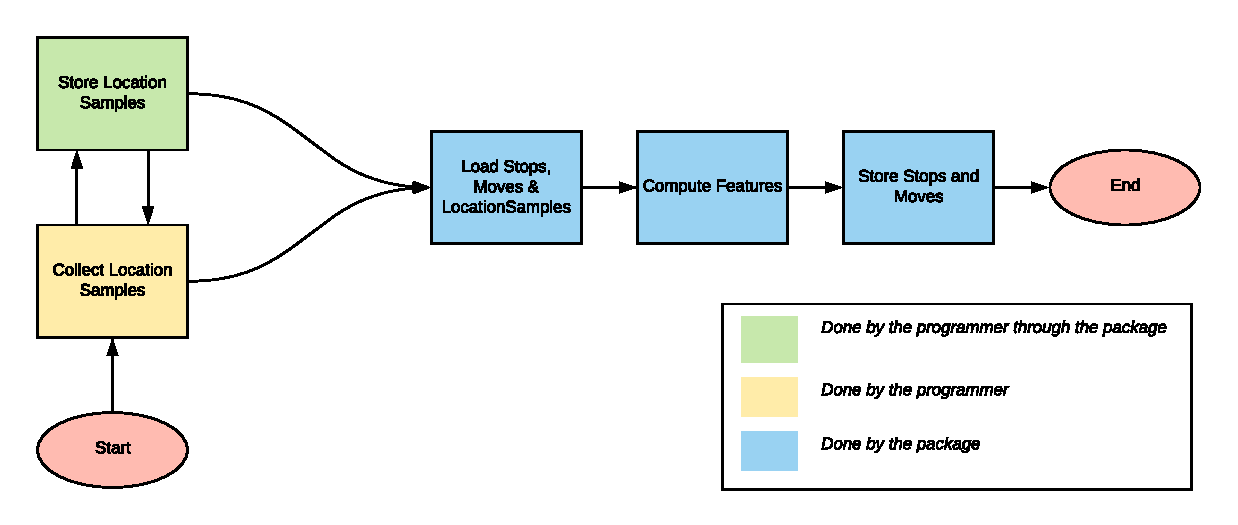
\includegraphics[width=0.5\textwidth]{images/diagrams/flowchart.pdf}
    \caption{Flowchart of the feature computatation process}
    \label{fig:my_label}
\end{figure}


\subsection{Component Overview}
Figure \ref{fig:component-diagram-internal} displays how the final iteration looks like as a software system: The main component is the \textit{Context Generator} component which is the interface that the programmer will use. This component exposes two interfaces to the programmer allowing the user to store their collected \textit{LocationSamples} as well as generate a \textit{Mobility Context} that contains the daily features. The two exposed interfaces are provided by the programmer through mobile application. The \textit{Context Generator} is also responsible for storing and loading data via the \textit{Mobility Serializer} component, here the \textit{Serializable} type refers to any data type that needs to be stored as historical data.

\begin{figure}[h]
\centering
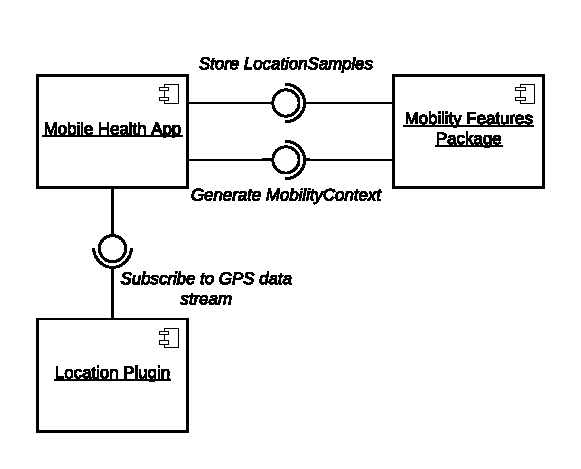
\includegraphics[width=0.5\textwidth]{images/diagrams/component-external.pdf}
\caption{Component diagram for the \textit{Mobility Feature Package} from an internal point of view}
\label{fig:component-diagram-internal}
\end{figure}

Figure \ref{fig:component-diagram-external} shows the external software system that includes the mobile application using the package. Another design choice is reflected in this figure which is the usage of an external location plugin which must be done by the programmer. This means task the programmer has to collect their own location data through their location plugin which will collect location \textit{Data Transfer Objects} (DTOs) \cite{fowler-PEEA} [p. 401]. These objects hold location data, i.e. latitude, longitude, and a timestamp and can be converted to \textit{LocationSamples} and saved through the \textit{Mobility Feature Package.}
Two reasons led to this decision, the first of which being that the Mobility Features Package becomes more loosely coupled and modular. The second reason relates to maintenance; if the package was to implement location data collection then it becomes harder to maintain since any change to the location plugin would imply changes to the Mobility Features Package as well. 

\begin{figure}[h]
\centering
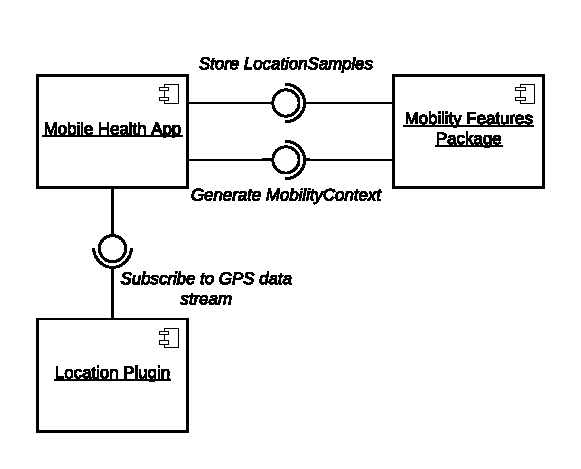
\includegraphics[width=0.5\textwidth]{images/diagrams/component-external.pdf}
\caption{Component diagram for the \textit{Mobility Feature Package} from an internal point of view}
\label{fig:component-diagram-external}
\end{figure}


\subsection{Sequence Overview}
To display the interactions between the components, sequence diagrams are used. Figure \ref{fig:sequence-diagram-external} shows the system from an external point of view, where the application subscribes to location updates via the location plugin, saves location data via the Mobility Features Package and generates a Mobility Context through it. 

\begin{figure}[h]
\centering
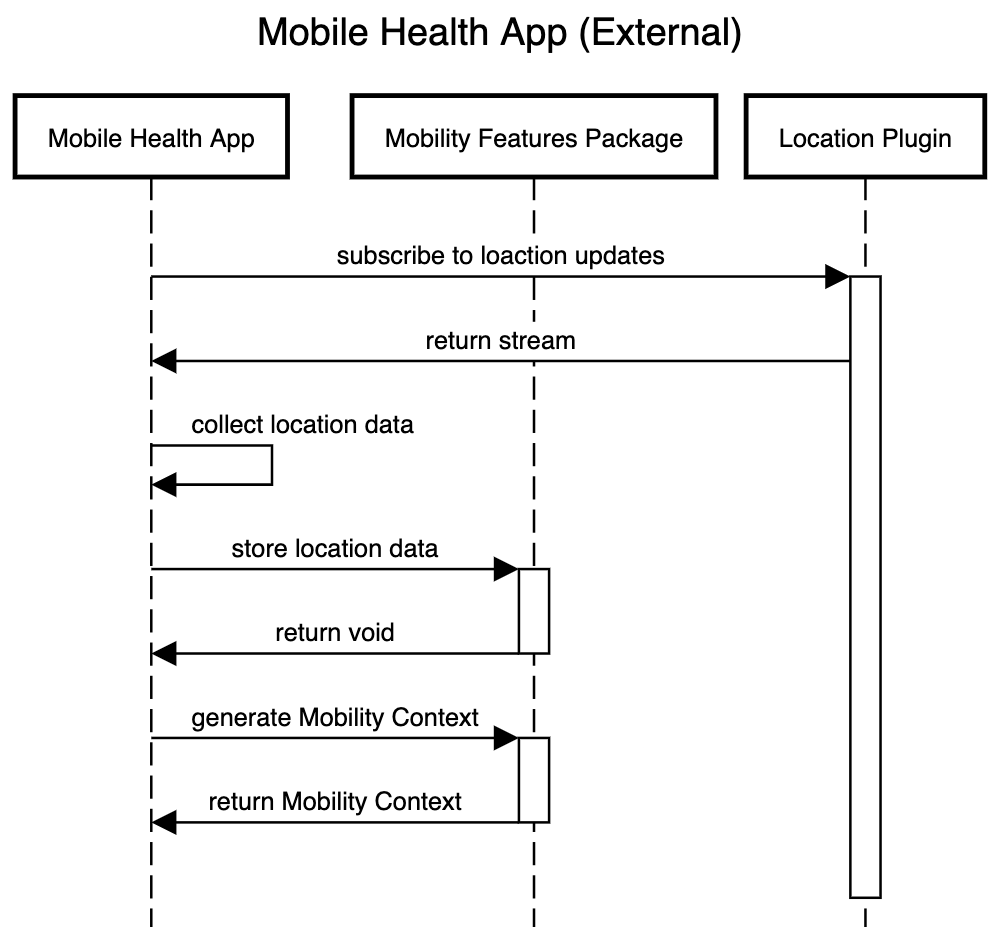
\includegraphics[width=0.7\textwidth]{images/diagrams/sequence-external.png}
\caption{Component diagram for the \textit{Mobility Feature Package} from an internal point of view}
\label{fig:sequence-diagram-internal}
\end{figure}

From an internal point of view, the \textit{Context Generator} component calls the \textit{Mobility Serializer} for storing and loading historical data, uses the loaded data to generate a \textit{Mobility Context} by calling the MobilityContext component.
\begin{figure}[h]
\centering
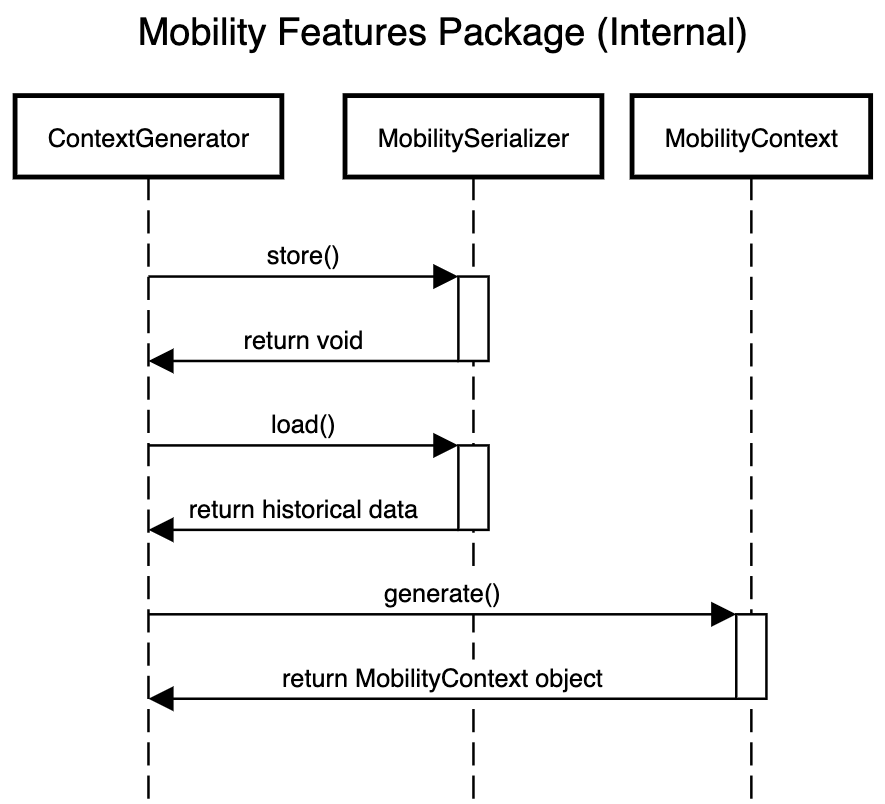
\includegraphics[width=0.7\textwidth]{images/diagrams/sequence-internal.png}
\caption{Sequence diagram for mobile health application using the Mobility Features Package, i.e. viewed externally from the package}
\label{fig:sequence-diagram-external}
\end{figure}
\section{Domain Model}
The domain model provides clarity and direction for a software system, even on a small scale such as in a library. In this section the design choices of the data model will be discussed.

\subsection{Data Model Overview}
In order to capture the data model in an object-oriented programming language, a UML diagram was maintained as the implementation went along in order to keep track of relationships between the classes. 
% As a general rule of thumb, all the fields were made public including those required by the constructors, and the methods of the classes were all \textit{getters}, i.e. \\

\subsubsection*{GeoPosition}
A \textit{GeoPosition} is defined by a geographical \textit{latitude} and \textit{longitude} and represents a 2D position on the Earth's surface.

\subsubsection*{Location Sample}
A \textit{Single Location Data Point} is a time-stamped \textit{Location}. By having a time-stamp, a collection of Location Samples may be ordered and grouped by the time of day. In essence, the class is a Data Transfer Object (DTO) \footnote{\url{https://martinfowler.com/eaaCatalog/dataTransferObject.html}} which is used to transfer GPS data from an arbitrary Location plugin to the \textit{Mobility Features Package}.

\subsubsection*{Hour Matrix}
An \textit{Hour Matrix} is a matrix with 24 rows and columns equal to the number of places of some period. The \textit{Hour Matrix} class is used to calculate the \textit{Routine Index} feature, as well as to identify the \textit{Home Cluster}, which is the place most visited during 00:00 and 06:00. An Hour Matrix is constructed from a list of \textit{Stops} which all have the same date.

\subsubsection*{Stop}
A \textit{Stop} is constructed from a centroid of a data point cluster (i.e. a Location) in addition to an arrival- and a departure timestamp, and a place ID indicating which place it belongs to.

\subsubsection*{Place}
A \textit{Place} is constructed from a place ID, as well as a collection of \textit{Stops} belonging to that \textit{Place}. 

\subsubsection*{Move}
A \textit{Move} is constructed from a pair of \textit{Stops} as well as the set of \textit{LocationSamples} which were sampled in between the two \textit{Stops} which is the path the user took between the two \textit{Stops}.

\subsubsection*{Mobility Context}
A \textit{Mobility Context} is a collection of features which are derived from a set of intermediate features, where the \textit{Stops} and \textit{Moves} are from a specific date. The \textit{Places} is derived from multiple dates for reasons which will be explained in the implementation details. In addition, a set of \textit{Mobility Contexts} from previous dates can be provided as an optional parameter. A Mobility Context contains the mobility features, although the \textit{Routine Index} is only available if an array of the set of \textit{Mobility Contexts} was provided as a parameter, which is due to the feature depending on the data from previous days in order to compare them.

\subsubsection*{GeoSpatial (Interface)}
This interface will impose a getter-method for the GeoPosition of the class which implements it. This allows the Haversine distance to be calculated between objects of different types.

\subsubsection*{Serializable (Interface)}
This interface will impose a serialization and de-serialization method for converting between a language object and a JSON object. The interface will allow the MobilitySerializer component as previosly discussed to more easily implement serialization in a generic manner which is disucssed in Chapter \ref{chapter:05}.

\subsection{UML Diagram and Discussion}

\begin{figure}[h]
    \centering
    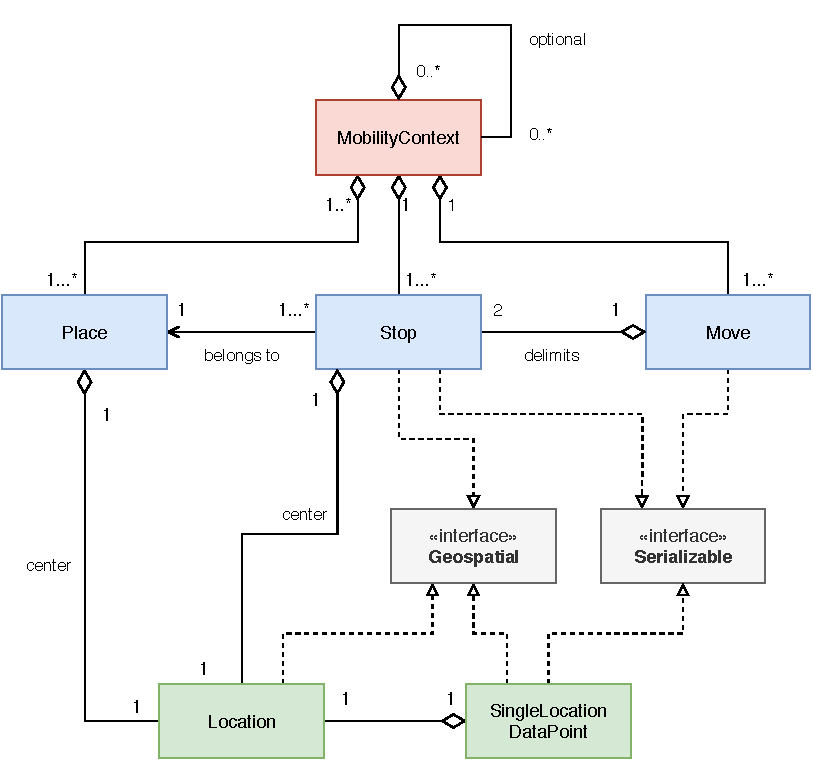
\includegraphics[width=0.7\textwidth]{images/diagrams/uml.pdf}
    \caption{UML diagram for the classes used in the \textit{Mobility Features Package}}
    \label{fig:my_label}
\end{figure}

The data model could be modified such that a Place contained a list of \textit{Stops} made at that place, rather than using both \textit{Places} and \textit{Stops} for instantiation of \textit{Mobility Context}. This would mean grouping the \textit{Stops} by Place rather than date, and would require filtering to take place every time a \textit{Mobility Context} object is created, to remove all Stops, not on that specific date. In a real-world scenario the application developer will likely have the Location Samples for the current day available, and from those the \textit{Stops} today can be generated which means no filtering is required. Grouping \textit{Stops} into places would however lead to a nicer data model, but a design choice was made in favor of less computation. 



\section{Requirements and Design Choices}
The functional requirements the package should meet and how these are met will be described in this section. Functionally speaking, the package should support the computation of the features described in \ref{chapter:03} however there are several layers to achieving this, including the following:

\begin{itemize}
    \item Save/Load location samples on device
    \item Compute intermediate features
    \item Save/Load Stops and Moves on Device
    \item Compute Mobility Features at any time (real-time)
\end{itemize}

Saving and loading of location samples was a necessity in order to not lose data: When an application tracks location data for a pro-longed period of time, i.e. a whole day, it will be sub-optimal to keep all the collected data in RAM, and thereby risking losing it if the app is killed by accident either by the OS or the user. Ideally, for storing the data points collected throughout the day a buffer of data points can be used which, once overflowed will store its elements to the disk. It was also necessary to store Stops and Moves on the device, such that which rely on historic data can be computed in the future. Therefore an interface for easily saving location data points was made, which also allowed the application programmer to load these data points whenever they were required for computation. 

\subsection{Serialization and JSON}
In order to save the SingleLocationPoints from today and historical Stops and Moves on the device they must be transformed from Dart objects into a data format which can store the state of the object, i.e. the information contained within it. The process of doing so is serialization and in this case Dart objects were transformed into JavaScript Object Notation (JSON) objects, which is a very common, human-readable data format that uses key-value pairs to store data. A JSON object can be stored in a database, or it can be transformed to a string in order to be stored. It was chosen to simply transform JSON objects to a string and write them to a local file, rather than storing the information in a database on the phone. The database approach is more involved and was therefore not chosen given the small scope of the project and working from a philosophy of getting a prototype up and running as fast as possible.

JSON supports a limited number of data types, such as strings, numbers, booleans, arrays, objects and null values. This means that in order to translate a Dart object to JSON, all of its fields must be serializable. An example of where this quickly becomes a problem, is with objects such as DateTime objects, since they are not supported by JSON - however a DateTime can be transformed to a number, which is milliseconds since epoch, or to an ISO standard date string. The approach is therefore to look at all the fields of the object that is to be serialized, and ensure that types of these fields all support some form of serialization. If they do not, it must be implemented.

\begin{figure}
    \centering
\begin{minted}{json}
{
    "location": {
        "latitude": 55.11787166161895,
        "longitude": 14.703046919371356
        },
    "datetime": "1586527196999"
}
\end{minted}
    \caption{Example of a serialized SingleLocationDataPoint}
    \label{fig:serialized_point}
\end{figure}

\begin{figure}
    \centering
\begin{minted}{json}
{
    "centroid": {
        "latitude": 55.11787908183754,
        "longitude": 14.703028176721789
        },
    "place_id": 0,
    "arrival": 1586556000999,
    "departure": 1586556697999
}
\end{minted}
    \caption{Example of a serialized Stop}
    \label{fig:serialized_stop}
\end{figure}

\begin{figure}
    \centering
\begin{minted}{json}
{
    "stop_from": {
        "centroid": {
            "latitude": 55.11053332998761,
            "longitude": 14.712282829580444
            },
        "place_id": 6,
        "arrival": 1586694154999,
        "departure": 1586696052001
    },
    "stop_to": {
        "centroid": {
            "latitude": 55.11793063393585,
            "longitude": 14.702982994031046
        },
        "place_id": 0,
        "arrival": 1586697230006,
        "departure": 1586699246824
    },
    "distance":2357.3408321427805
}
\end{minted}
    \caption{Example of a serialized Move}
    \label{fig:serialized_move}
\end{figure}


For loading an object from disk into application memory again it must also support de-serialization which reads values of the JSON object's keys and stores them in a Dart object. If we continue the example of a DateTime object which was serialized by either converting it to a number or a string, de-serialization must use a parser which reads the string bit by bit or use some math for calculating what day a time delta from January 1st 1970 is. 

Serialization and de-serialization is implemented by making an abstract class called Serializable, which has two functions: toJson and fromJson. The toJson function converts the object itself to a JSON object and the fromJson function is a so-called factory function which is in essence a constructor which creates a Dart object given a JSON object. The SingleLocationPoint, Stop and Move classes all implement the Serializable interface, which requires the classes to have a concrete implementation of these two methods, which in turn ensures the compiler that all of these classes can be serialized and de-serialized, which makes generalizing about objects belonging to either of these classes easier. Concretely, a generic class, Serializer<E>, was implemented in order to handle serialization, in which a type E is specified, which must a Serializable class. This makes it efficient in terms of lines of code to serialize a list of objects, since they are all required to implement toJson method, which produces a JSON object, and for de-serialization purposes they can all be constructed from a JSON object, given that it contains a set of correctly formatted key-value pairs.




